\documentclass[12pt, titlepage]{article}

\usepackage{fullpage}
\usepackage[round]{natbib}
\usepackage{multirow}
\usepackage{booktabs}
\usepackage{tabularx}
\usepackage{graphicx}
\usepackage{float}
\usepackage{xr}
\usepackage{xr-hyper}
\usepackage{hyperref}
\hypersetup{
    colorlinks,
    citecolor=blue,
    filecolor=black,
    linkcolor=red,
    urlcolor=blue
}

\usepackage[round]{natbib}
\usepackage{longtable}
\usepackage[utf8]{inputenc}
\usepackage{amsmath, mathtools}
\usepackage{amsfonts}
\usepackage{amssymb}
\usepackage{colortbl}
\usepackage{longtable}
\usepackage{xfrac}
\usepackage{siunitx}
\usepackage{caption}
\usepackage{pdflscape}
\usepackage{afterpage}
\usepackage{seqsplit}
\usepackage{underscore}
\usepackage{lscape}
\usepackage[english]{babel}
\usepackage[T1]{fontenc}
\usepackage{nameref}
\usepackage{enumitem}
\usepackage{gensymb}

%% Comments

\usepackage{color}

\newif\ifcomments\commentstrue %displays comments
%\newif\ifcomments\commentsfalse %so that comments do not display

\ifcomments
\newcommand{\authornote}[3]{\textcolor{#1}{[#3 ---#2]}}
\newcommand{\todo}[1]{\textcolor{red}{[TODO: #1]}}
\else
\newcommand{\authornote}[3]{}
\newcommand{\todo}[1]{}
\fi

\newcommand{\wss}[1]{\authornote{blue}{SS}{#1}} 
\newcommand{\plt}[1]{\authornote{magenta}{TPLT}{#1}} %For explanation of the template
\newcommand{\an}[1]{\authornote{cyan}{Author}{#1}}

%% Common Parts

\newcommand{\progname}{Mechatronics Engineering} % PUT YOUR PROGRAM NAME HERE
\newcommand{\authname}{Team \# 34, ParkingLotHawk
\\ Fady Zekry Hanna, zekryhf
\\ Winnie Trandinh, trandint
\\ Muhammad Ali, alim102
\\ Muhammad Khan, khanm120} % AUTHOR NAMES                  

\usepackage{hyperref}
    \hypersetup{colorlinks=true, linkcolor=blue, citecolor=blue, filecolor=blue,
                urlcolor=blue, unicode=false}
    \urlstyle{same}
                                

%\externaldocument{../DevelopmentPlan/DevelopmentPlan}
\externaldocument{../HazardAnalysis/HazardAnalysis}
\externaldocument{../SRS/SRS}
\externaldocument{../VnVPlan/VnVPlan}
%\externaldocument{../Design/SoftDetailedDes/MIS}
%\externaldocument{../Design/SoftArchitecture/MG}
\externaldocument{../UserManual/UserManual}

\begin{document}

\title{Verification and Validation Report: \progname} 
\author{\authname}
\date{\today}
	
\maketitle

\pagenumbering{roman}

\section{Revision History}

\begin{tabularx}{\textwidth}{p{3cm}p{2cm}X}
\toprule {\bf Date} & {\bf Version} & {\bf Notes}\\
\midrule
March 8, 2023 & 1.0 & Initial Revision \\
\bottomrule
\end{tabularx}

~\newpage

\section{Definitions, Abbreviations, and Acronyms}
\label{sec:defAbrev}

\renewcommand{\arraystretch}{1.2}
\begin{tabular}{l l} 
  \toprule		
  \textbf{symbol} & \textbf{description}\\
  \midrule 
  Fail & None of the test case's purpose was verified. \\
  FR & Functional Requirement \\
  FSM & Finite State Machine \\
  NFR & Non Functional Requirement \\
  Partially Pass & A part of the test case's purpose was verified, but another part was not. \\
  Pass & Expected and actual results of the test case match. \\
  Principally Pass & The purpose of the test case is verified in a similar/modified test. \\
  SITL & Software in The Loop \\
  SRS & Software Requirement Specifications \\
  VnV & Verification and Validation \\
  \bottomrule
\end{tabular}\\

\newpage

\tableofcontents

\listoftables %if appropriate

\listoffigures %if appropriate

\newpage

\pagenumbering{arabic}

\section{Design Verification}
\label{sec:designVerification}
As outlined within the \nameref{vnvPlan}, multiple methods are utilized to verify the SRS and design to ensure that the design is meeting the requirements. This is done by verifying the SRS, the design, and then the VnV Plan itself.

\subsection{SRS Verification}
\label{subsec:srsVerification}
The Finite State Machine (FSM) outlined within the Software Requirement Specifications (SRS) has been formally verified through the maintenance of a decision table, located within \nameref{appendixb}. Through informal verification, the team has conducted a guided review with a technical external party, using the process outlined within the \nameref{SRSVerification}. All Nonfunctional Requirements (NFRs) mentioned by the external party are present within the SRS, with additional NFRs not mentioned by the external party. These NFRs were discussed to determine if they are required, and no changes were made to the SRS as a result. 

The checklist outlined within the \nameref{SRS_Checklist} has also been conducted internally within the team and all points have been met. Furthermore, a code review has been conducted within the team to recreate the FSM from just the code. The resulting FSM matches the one located within \nameref{appendixb}, thus ensuring that the FSM is correctly implemented.

\subsection{Design Verification}
\label{subsec:designVerification}
The Design Verification consists of a guided review with and external party, using the checklist provided within the \nameref{Design1_Checklist} as a reference. The main purpose is to ensure that all Functional Requirements (FRs) have been met. The results of the review can be found in \nameref{tab:extDesignVerification}. For conciseness, points that have been met and has no additional feedback are excluded in the results.

\begin{table}[!h]
\begin{center}
\caption {External Design Verification}
\label{tab:extDesignVerification}
\begin{tabular}{ | m{5.2cm} | m{5.2cm} | m{5.0cm} | } 
\hline
Criteria & Feedback & Team Response \\ 
\hline
The condition i\_MinHoverHeight <= i\_DesiredHoverHeight <= i\_MaxHoverHeight shall always be true. & 
    This requirement is not explicitly associated with a specific module or state, whether it's the GUI module or the Configure State. Thus, no module is currently verifying this condition. &
    The condition will be verified within the Configure State when the values are updated by the user. \\ 
\hline
The product shall be shall highlight non-occupied parking slots on the operator's display (update c\_CurrentView). &
    There is no window to show the c\_currentView. Only the live camera output is visible. &
    The new window will be added into the GUI module. \\
\hline
\end{tabular}
\end{center}
\end{table}

\clearpage

A more detailed internal review has also been conducted using \nameref{Design2_Checklist}, with the results in \nameref{tab:intDesignVerification}.

\begin{table}[!h]
\begin{center}
\caption {Internal Design Verification}
\label{tab:intDesignVerification}
\begin{tabular}{ | m{7.7cm} | m{7.7cm} | } 
\hline
Criteria & Feedback \\ 
\hline
Does the design implement all the performance requirements listed below? & 
    These requirements have not been fully tested in the real world. However, all performance requirements have been tested within a Software in The Loop (SITL) environment and has met all requirements. \\ 
\hline
The product shall be mechanically waterproof, to the point it can sustain a light drizzle for 1 minute of operation while still performing within the requirements. &
    The product has not been explicitly tested within the rain for operation, but design considerations have been made to mechanically isolate the electronic components. The product is capable of aerial flight during light snow flurries and takeoff/landing in 5cm+ of frozen snow. \\
\hline
The product shall be able to operate and provide data to the operator for > 5 minutes without the need to recharge. &
    The product is currently capable of only 3.5 minutes of flight outdoors. However, this degradation in battery capacity is due to the cold weather during testing (-5\degree C and below) and its negative impact on LiPo battery performance. \\
\hline
\end{tabular}
\end{center}
\end{table}

\clearpage

\subsection{Verification and Validation Plan Verification}
\label{subsec:vnvVerification}

The VnV Plan has been verified through a review process with an external Capstone group, using the  \nameref{VnV_Checklist}. All points have been met. However, the external party has noted that there are too many test cases given the flight time of 5 minutes, thus making the tests difficult to execute and would require multiple batteries to be swapped and recharged. Therefore, the team will consider using a larger battery capacity for future iterations.


\section{System Testing}
\label{sec:SystemTesting}

This section contains the results of the System Tests outlined within \nameref{systemTest}. Detailed test procedures can be found within the Test Case Reference provided within the results. Each test case is then either evaluated as a Pass, Principally Pass, Partially Pass, or Fail, as defined within \nameref{sec:defAbrev}. Some test cases use the SITL environment as defined within \nameref{subsec:sitl}.

\subsection{Flight Dynamics}

\begin{table}[!h]
\begin{center}
\caption {STCR\_001}
\label{tab:STCR_001}
\begin{tabular}{ | m{3.2cm} | m{12.2cm} | } 
\hline
Test Case Result ID & \nameref{tab:STCR_001} \\ 
\hline
Test Case Reference & \nameref{tab:STC_001}  \\ 
\hline
Requirements Tested & \nameref{GEN_003}, \nameref{GEN_004}, \nameref{STA_000}, \nameref{STA_001}, \nameref{STA_004}, \nameref{STA_005}, \nameref{STA_006}, \nameref{TRANS_002}, \nameref{TRANS_003}, \nameref{TRANS_009}, \nameref{PERF_002} \\ 
\hline
Procedure & Fly the drone indoors in its hovering state for a minute. \\ 
\hline
Expected Result & The drone should reach its hover height within 25 seconds, and hover within 0.5m of the requested hovering height. The drone should also stay within 1.5m of the launch location.  \\ 
\hline
Actual Result & The drone was flown outdoors using an RC Controller in a guided control mode(i.e. the Parking Lot Hawk which autonomously flies the drone was not used). Within this mode, altitude and location are maintained when no user inputs are given. It successfully flew for 60 seconds and took off in less than 25 seconds. No additional movement commands were sent after takeoff, and the drone maintained a 1.5m radius around the launch location, and height was maintained within 0.5m.  \\ 
\hline
Result Analysis & Pass. The purpose of this test was to verify that the drone is mechanically and electrically able to take off and maintain flight in a simple no-wind indoor scenario. By hovering outdoors (with wind gusts) for 60 seconds, the essence of the test was verified on a more difficult scenario.  \\ 
\hline
\end{tabular}
\end{center}
\end{table}




\begin{table}[!h]
\begin{center}
\caption {STCR\_002}
\label{tab:STCR_002}
\begin{tabular}{ | m{3.2cm} | m{12.2cm} | } 
\hline
Test Case Result ID & \nameref{tab:STCR_002} \\ 
\hline
Test Case Reference & \nameref{tab:STC_002}  \\ 
\hline
Requirements Tested & \nameref{SAFE_002}, \nameref{GEN_004} \\ 
\hline
Procedure & Attempt to set the height parameters of the drone to invalid values. First, try to set them to be below the minimum height requirement (7m), then try to set the maximum hover height to be less than the minimum hover height.  \\ 
\hline
Expected Result & The drone should prevent the user from entering invalid height parameters both times, and return an error that the height parameters are invalid.   \\ 
\hline
Actual Result & The drone does not fulfill the user's request to set the height parameters, and an error message is logged in the GUI log box.  \\ 
\hline
Result Analysis & Pass.  \\ 
\hline
\end{tabular}
\end{center}
\end{table}




\begin{table}[!h]
\begin{center}
\caption {STCR\_003}
\label{tab:STCR_003}
\begin{tabular}{ | m{3.2cm} | m{12.2cm} | } 
\hline
Test Case Result ID & \nameref{tab:STCR_003} \\ 
\hline
Test Case Reference & \nameref{tab:STC_003}  \\ 
\hline
Requirements Tested & \nameref{GEN_003}, \nameref{GEN_004}, \nameref{STA_000}, \nameref{STA_001}, \nameref{STA_004}, \nameref{STA_005}, \nameref{STA_006}, \nameref{TRANS_002}, \nameref{TRANS_003}, \nameref{TRANS_009}, \nameref{PERF_002} \\ 
\hline
Procedure & Attempt to take off and hover the drone at the minimum safe hover height (7m) for 60 seconds. After the test, land the drone by asserting m\_land. \\ 
\hline
Expected Result & The drone should launch to 7m within 25 seconds, hover within 0.5m of the 7m height, and laterally stay within 1.5m of the launch location.   \\ 
\hline
Actual Result & Within SITL, the drone successfully takes off to 7m. It successfully remains within the height and lateral requirements for the time period specified. The test was never performed with the physical drone in an outdoor environment.  \\ 
\hline
Result Analysis & Partially Pass. One of the purposes of the test was to verify operation states (such as configure, hover, and land). The SITL test verified the operation states. The test's primary purpose was to verify that the drone's mechanical design, electrical design, and autonomous flight software can fly and land the drone from a height of 7m. The product failed to fulfill the primary purpose of this test. The cause of failure is that the autonomous flight software has not yet been fully tuned, thus autonomous flight cannot be performed. See \nameref{tab:STCR_001} for a test of the product's mechanical and electrical design.  \\ 
\hline
\end{tabular}
\end{center}
\end{table}





\begin{table}[!h]
\begin{center}
\caption {STCR\_004}
\label{tab:STCR_004}
\begin{tabular}{ | m{3.2cm} | m{12.2cm} | } 
\hline
Test Case Result ID & \nameref{tab:STCR_004} \\ 
\hline
Test Case Reference & \nameref{tab:STC_004}  \\ 
\hline
Requirements Tested & \nameref{STA_002}, \nameref{TRANS_005}, \nameref{PERF_008}, \nameref{PERF_006}, \nameref{USE_001}, \nameref{PERF_003}
\\ 
\hline


\hline
Procedure & While in a flight state, set the desired location to be 20m diagonally forward-right, and enter the compulsive move state (by asserting m\_CompulsiveMove).    \\ 
\hline
Expected Result & The drone should fly toward the desired location, traveling at least 4 m/sec. A live display of the drone's location and a visual trace of the drone's past location should be visible in the GUI. After reaching the desired location, the drone should remain within 1.5m of the desired location.    \\ 
\hline
Actual Result & Within SITL, the drone successfully flies in a straight line path to the desired location, while satisfying the height, speed, and lateral position requirements. The test was never performed with the physical drone in an outdoor environment. \\ 
\hline
Result Analysis & Partially Pass. One of the purposes of the test was to verify the compulsive move operation states. The SITL test verifies that operation state. The test's primary purpose however was to verify that the drone's mechanical design, electrical design, and autonomous flight software can laterally fly the drone and fly faster than the 4 m/sec average speed requirement. The product failed to fulfill the primary purpose of this test. The cause of failure is that the autonomous flight software has not yet been fully tuned, thus autonomous flight cannot be performed. \\ 
\hline
\end{tabular}
\end{center}
\end{table}

\clearpage

\subsection{Battery}


\begin{table}[!h]
\begin{center}
\caption {STCR\_005}
\label{tab:STCR_005}
\begin{tabular}{ | m{3.2cm} | m{12.2cm} | } 
\hline
Test Case Result ID & \nameref{tab:STCR_005} \\ 
\hline
Test Case Reference & \nameref{tab:STC_005}  \\ 
\hline
Requirements Tested & \nameref{SR_003} \\ 
\hline
Procedure & Compare the battery capacity displayed on the GUI with the actual battery capacity (obtained by connecting the battery to its charger).  \\ 
\hline
Expected Result & The battery capacity displayed on the GUI should match the true battery capacity displayed on the charger.   \\ 
\hline
Actual Result & The GUI's battery capacity is 2\% less than the true battery capacity.  \\ 
\hline
Result Analysis & Pass, the battery capacity error is negligible.  \\ 
\hline
\end{tabular}
\end{center}
\end{table}

\begin{table}[!h]
\begin{center}
\caption {STCR\_006}
\label{tab:STCR_006}
\begin{tabular}{ | m{3.2cm} | m{12.2cm} | } 
\hline
Test Case Result ID & \nameref{tab:STCR_006} \\ 
\hline
Test Case Reference & \nameref{tab:STC_006}  \\ 
\hline
Requirements Tested & \nameref{SR_011}, \nameref{STA_009}\, \nameref{USE_003}, \nameref{SR_003}
\\  
\hline
Procedure &  Fly the drone in any flying state.  \\ 
\hline
Expected Result & After a sufficiently long time (at least 3.5 minutes), when the battery capacity remaining is less than 1.5 minutes, the drone will enter the Malfunction state. Upon entering the malfunction state, the drone shall log an error message and land itself at its original launch location.   \\ 
\hline
Actual Result & Within the SITL, the drone enters the Malfunction state after 6 minutes of flight. The battery capacity remaining at his point is 20\% (1.5 minutes). The drone logs a low battery message and lands at its launch location. The test was never performed with the physical drone in an outdoor environment. \\ 
\hline
Result Analysis & Partially Pass. The primary purpose of the test was to verify the Malfunction state and the low battery transitions. The SITL test verifies the Malfunction state and the low battery transition. The test's secondary purpose however was to verify that the drone's mechanical design and electrical design allow a battery life of flight time of at least 3.5 minutes. The product failed to fulfill the secondary purpose of this test. The cause of failure is that the autonomous flight software has not yet been fully tuned, thus autonomous flight cannot be performed. \\ 
\hline
\end{tabular}
\end{center}
\end{table}


\begin{table}[!h]
\begin{center}
\caption {STCR\_007}
\label{tab:STCR_007}
\begin{tabular}{ | m{3.2cm} | m{12.2cm} | } 
\hline
Test Case Result ID & \nameref{tab:STCR_007} \\ 
\hline
Test Case Reference & \nameref{tab:STC_007}  \\ 
\hline
Requirements Tested & \nameref{SR_012} \\ 
\hline
Procedure & Attempt to launch the drone when the battery remaining is less than 3 minutes of flight.  \\ 
\hline
Expected Result & The drone does not launch and instead returns a descriptive error message.   \\ 
\hline
Actual Result & The drone remains in the Idle state (does not launch). A low battery error message is seen in the GUI's log box.  \\
\hline
Result Analysis & Pass. \\ 
\hline
\end{tabular}
\end{center}
\end{table}

\clearpage

\subsection{Communication}

\begin{table}[!h]
\begin{center}
\caption {STCR\_008}
\label{tab:STCR_008}
\begin{tabular}{ | m{3.2cm} | m{12.2cm} | } 
\hline
Test Case Result ID & \nameref{tab:STCR_008} \\ 
\hline
Test Case Reference & \nameref{tab:STC_008}  \\ 
\hline
Requirements Tested & \nameref{STA_010}, \nameref{TRANS_010}
\\ 
\hline
Procedure & During any of the flight states, disconnect the Operator's PC from the Wifi communication network.     \\ 
\hline
Expected Result & The drone should log an error message, return an unhealthy status, and enter the communication lost state.   \\ 
\hline
Actual Result & Within SITL, the drone enters the Communication Lost state and lands upon the communication network being disconnected. A log message and unhealthy status is seen on the Operator's PC. While testing on the drone but with propellers disconnected and in a flight state, it is observed that the drone enters the Communication Lost state.  \\ 
\hline
Result Analysis & Principally Pass. The purpose of this test was to verify the Communication Lost state. The operation of the communication lost state was verified in SITL, and the transition into the state was verified using the stationary drone test. Thus the purpose of this test was accomplished. The purpose of this test did not mention any flight dynamics testing, as there are other test cases to verify landing dynamics (\nameref{tab:STCR_003}), thus a real-life flight is not necessary.   \\ 
\hline
\end{tabular}
\end{center}
\end{table}



\begin{table}[!h]
\begin{center}
\caption {STCR\_009}
\label{tab:STCR_009}
\begin{tabular}{ | m{3.2cm} | m{12.2cm} | } 
\hline
Test Case Result ID & \nameref{tab:STCR_009} \\ 
\hline
Test Case Reference & \nameref{tab:STC_009}  \\ 
\hline
Requirements Tested & \nameref{STA_010}, \nameref{TRANS_010} 

\\  
\hline
Procedure & During any of the flight states, close the Parking Lot Hawk application running on the Operator's PC.     \\ 
\hline
Expected Result & The drone should log an error message, return an unhealthy status, and enter the communication lost state.   \\ 
\hline
Actual Result & Within SITL, the drone enters the Communication Lost state and lands upon the application being closed. A log message and unhealthy status were seen on the Operator's PC. While testing on the drone but with propellers disconnected and in a flight state, it is observed that the drone enters the Communication Lost state.  \\ 
\hline
Result Analysis & Principally Pass. The purpose of this test was to verify that the drone correctly transitions to the Communication Lost state when the Parking Lot Hawk application is closed, and verify the operation of the Communication Lost state. The operation of the communication lost state was verified in SITL, and the transition into the state was verified using the stationary drone test. Thus the purpose of this test was accomplished. The purpose of this test did not mention any flight dynamics testing, as there are other test cases to verify landing dynamics (\nameref{tab:STCR_003}), thus a real-life flight is not necessary.   \\ 
\hline
\end{tabular}
\end{center}
\end{table}


\begin{table}[!h]
\begin{center}
\caption {STCR\_010}
\label{tab:STCR_010}
\begin{tabular}{ | m{3.2cm} | m{12.2cm} | } 
\hline
Test Case Result ID & \nameref{tab:STCR_010} \\ 
\hline
Test Case Reference & \nameref{tab:STC_010}  \\ 
\hline
Requirements Tested & \nameref{SR_007}, \nameref{STA_010}, \nameref{TRANS_010} \\

\hline
Procedure & Fly the drone forward until Communication is lost, which can be done by choosing a far away desired location and using Compulsive Move.   \\
\hline
Expected Result & Upon communication being lost, the drone should enter the Communication Lost state and fly back toward the launch location. While flying back the drone should eventually reconnect to the Operator's PC, and enter the Hover state.    \\ 
\hline
Actual Result & The test was performed with the propellers disconnected, and a person holding and walking with the drone away. The drone lost communication at about 200m. When the tester walked back, the drone reconnected and entered the Hover state. 

The test was not performed in proper flight as the drone has not yet been tuned for autonomous flight. The test could not be performed in SITL either, as even at large distances the simulated drone would not lose connection.  \\
\hline
Result Analysis & Partially Pass. The primary purpose of the test was to stress test the strength of the communication network and the ability of the drone to disconnect and reconnect. Another reason for the test is to verify transitions to and from Communication Lost state as well as its operation. Both purposes were fulfilled by the manual walking with the drone test. Another purpose of the test case was to elucidate how performance degrades with the drone far away. This purpose cannot be tested until the drone flies autonomously in the real physical world.  \\ 
\hline
\end{tabular}
\end{center}
\end{table}

\clearpage

\subsection{User Error States}

\begin{table}[!h]
\begin{center}
\caption {STCR\_011}
\label{tab:STCR_011}
\begin{tabular}{ | m{3.2cm} | m{12.2cm} | } 
\hline
Test Case Result ID & \nameref{tab:STCR_011} \\ 
\hline
Test Case Reference & \nameref{tab:STC_011}  \\ 
\hline
Requirements Tested & \nameref{STA_013}, \nameref{TRANS_005} \\ 
\hline
Procedure & Change m\_DesiredUserLocation to a location outside of the parking lot. Assert m\_CompulsiveMove to make the drone move to the desired location. A prompt will open asking if the user is sure they want the drone to move a location outside of a parking lot, respond with "OK". \\
\hline
Expected Result & When the user attempts to move to an invalid location, the ParkingLotHawk application running on the Operator's PC should display a prompt, indicating that the desired location is invalid. When the user presses "OK", indicating they still want to fly to the location, the drone should fly toward the desired location of the user.  \\ 
\hline
Actual Result & Within SITL, the drone gave a prompt informing the user the requested location is not within a parking lot. Upon selecting "Yes", the drone flied towards the requested location. The test was not performed in real life as the drone is still not tuned for autonomous flight.  \\
\hline
Result Analysis & Principally Pass. The purpose of the test was to verify the ability of the drone to prompt the user when the requested location is detected as invalid, this behavior was verified by the SITL test. The ability of the drone to detect parking boundaries was not a motivation for this test, and rather is the motivation for \nameref{tab:STC_014}.  \\ 
\hline
\end{tabular}
\end{center}
\end{table}


\begin{table}[!h]
\begin{center}
\caption {STCR\_012}
\label{tab:STCR_012}
\begin{tabular}{ | m{3.2cm} | m{12.2cm} | } 
\hline
Test Case Result ID & \nameref{tab:STCR_012} \\ 
\hline
Test Case Reference & \nameref{tab:STC_012}  \\ 
\hline
Requirements Tested & \nameref{STA_003}, \nameref{TRANS_004}, \nameref{STA_011}, \nameref{TRANS_012}, \nameref{STA_008}, \nameref{TRANS_008} \\ 

\\ 
\hline
Procedure & While flying in a non-parking lot area, attempt to enter the drone Autonomous Explore state. Then fly the drone to a location within the parking lot (using the Compulsive move feature) and attempt to enter the Autonomous Explore state.     \\
\hline
Expected Result & The first attempt to Autonomously Explore the parking lot should fail and the drone should enter the No Parking Lot Detected Error state. During this state, the drone should continuously hover, a descriptive error message should appear in c\_Log, and c\_UserError should change to No_Lot_Detected_State. During the Compulsive Move state, c_UserError should be None. The second attempt to enter the Autonomous Explore state should succeed.   \\ 
\hline
Actual Result & Within SITL, the first attempt to enter the Autonomous Explore state failed. The drone entered the No Parking Lot Error state when the desired location was not within a parking lot. During the No Parking Lot Detected state, the drone was hovering and an error message is seen in c\_Log, and c\_UserError is No_Lot_Detected_State. During the Compulsive Move state, c_UserError changed to None. The second attempt to enter the Autonomous Explore succeeded. The test was not performed in real life.  \\
\hline
Result Analysis & Principally Pass. The purpose of the test was to verify the transition to the Autonomous Explore state, verify the behavior of the compulsive move state moving to a location, and verify the behavior of the No Parking Lot Error state. These activities were verified by the SITL test. The ability of the drone to detect parking boundaries was not a motivation for this test, and rather is the motivation for \nameref{tab:STC_014}.   \\ 
\hline
\end{tabular}
\end{center}
\end{table}

\clearpage

\subsection{Visual Perception and Path Planning}

\begin{table}[!h]
\begin{center}
\caption {STCR\_013}
\label{tab:STCR_013}
\begin{tabular}{ | m{3.2cm} | m{12.2cm} | } 
\hline
Test Case Result ID & \nameref{tab:STCR_013} \\ 
\hline
Test Case Reference & \nameref{tab:STC_013}  \\ 
\hline
Requirements Tested & \nameref{GEN_005}, \nameref{GEN_006}, \nameref{STA_003}, \nameref{GEN_001}, \nameref{GEN_002}, \nameref{STA_003}, \nameref{TRANS_004}, \nameref{PERF_004}, \nameref{PERF_001} \\ 
\hline
Procedure & Place a fully charged drone within a small (~30 spots) rectangular shaped parking lot.  Launch the drone. \\
\hline
Expected Result & The drone should automatically detect the parking lot upon launch and enter the Autonomous Explore state. The drone should fully explore the parking lot within battery capacity. c\_CameraView should contain the live view of the drone's camera and should update at 0.5 FPS. The occupancy map should be completed with reasonable accuracy.  \\ 
\hline
Actual Result &  The test was not performed. \\
\hline
Result Analysis & Fail. The primary purpose of the test was to verify the operation of the  autonomous explore feature during a live real-life test case. SITL cannot be used for this test case because it is the motivation for a different test, \nameref{tab:STC_016}. The test was not performed in real life as the drone is still not tuned for autonomous flight.  \\ 
\hline
\end{tabular}
\end{center}
\end{table}



\begin{table}[!h]
\begin{center}
\caption {STCR\_014}
\label{tab:STCR_014}
\begin{tabular}{ | m{3.2cm} | m{12.2cm} | } 
\hline
Test Case Result ID & \nameref{tab:STCR_014} \\ 
\hline
Test Case Reference & \nameref{tab:STC_014}  \\ 
\hline
Requirements Tested & \nameref{GEN_001}, \nameref{SR_009}
\\ 
\hline
Procedure & Hold and carry the drone to an area that has grass, then to the middle of a roadway with lane markings, and finally move with the drone to a parking lot. \\
\hline
Expected Result & The Operator’s PC should display c_ParkLotDetected as false in all places except when the drone is inside a parking lot.   \\ 
\hline
Actual Result &  The Operator’s PC displayed c_ParkLotDetected as false in all
places except when the drone is inside a parking lot, where it was true.  \\
\hline
Result Analysis & Pass.  \\ 
\hline
\end{tabular}
\end{center}
\end{table}




\begin{table}[!h]
\begin{center}
\caption {STCR\_015}
\label{tab:STCR_015}
\begin{tabular}{ | m{3.2cm} | m{12.2cm} | } 
\hline
Test Case Result ID & \nameref{tab:STCR_015} \\ 
\hline
Test Case Reference & \nameref{tab:STC_015}  \\ 
\hline
Requirements Tested & \nameref{GEN_005}, \nameref{SR_009} \\ 
\hline
Procedure & Hold the drone over a printed picture of a parking lot. \\
\hline
Expected Result & c\_CurrentView should contain the printed image in its view.The drone should also identify if the location it is hovering over is occupied by an object or not.   \\ 
\hline
Actual Result &   c\_CurrentView contains the current image. It correctly detected if it was hovering over a vehicle or empty parking lot space.  \\
\hline
Result Analysis & Pass.  \\ 
\hline
\end{tabular}
\end{center}
\end{table}


\begin{table}[!h]
\begin{center}
\caption {STCR\_016}
\label{tab:STCR_016}
\begin{tabular}{ | m{3.2cm} | m{12.2cm} | } 
\hline
Test Case Result ID & \nameref{tab:STCR_016} \\ 
\hline
Test Case Reference & \nameref{tab:STC_016}  \\ 
\hline
Requirements Tested & \nameref{GEN_001}, \nameref{GEN_002}, \nameref{GEN_005}, \nameref{GEN_006}, \nameref{STA_003}, \nameref{TRANS_003}
\\ 
\hline
Procedure & Launch the drone within a custom-made 3D SITL environment with a small (~30 spaces) rectangular parking lot.  \\
\hline
Expected Result & The drone should automatically detect the parking lot upon launch, and enter the Autonomous Explore state. The drone should fully explore the parking lot. c\_CameraView should contain the live view of the drone's camera, and should update at 0.5 FPS. The occupancy map should be completed with reasonable accuracy.  \\ 
\hline
Actual Result &  The test was not performed. \\
\hline
Result Analysis & Fail. The primary purpose of the test was to verify the path planning/autonomous explore feature of the drone. The path planning feature was a stretch goal for this project and was not implemented, thus the Autonomous Explore state is empty (it simply hovers the drone).    \\ 
\hline
\end{tabular}
\end{center}
\end{table}

\clearpage

\subsection{User Manual}
The following tests were conducted with the \href{https://github.com/icecap360/DroneCapstone/blob/master/docs/UserManual/UserManual.pdf}{User Manual} that is included with the product.

\begin{table}[!h]
\begin{center}
\caption {STCR\_017}
\label{tab:STCR_017}
\begin{tabular}{ | m{3.2cm} | m{12.2cm} | } 
\hline
Test Case Result ID & \nameref{tab:STCR_017} \\ 
\hline
Test Case Reference & \nameref{tab:STC_017}  \\ 
\hline
Requirements Tested & \nameref{tab:STC_012}, \nameref{USE_004} 
\\ 
\hline
Procedure & Two volunteers who have never used Parking Lot Hawk before reads the user manual, attempt to install the Parking Lot Hawk application, and conduct test case \nameref{tab:STC_012} independently. \\
\hline
Expected Result & Both volunteers successfully install the application and complete \nameref{tab:STC_012} without any help from the developers within 2 hours.  \\ 
\hline
Actual Result &  The volunteers independently installed the Parking Lot Hawk Application and conducted the \nameref{tab:STC_012} within a premade SITL environment within 2 hours. \\
\hline
Result Analysis & Partially Pass. The primary purpose of the test was to verify that new users can learn to use the Parking Lot Hawk using just the user manual. Although users were able to install and use the drone in SITL, because they did not operate the drone in real-life the test cannot be declared as pass.    \\ 
\hline
\end{tabular}
\end{center}
\end{table}


\begin{table}[!h]
\begin{center}
\caption {STCR\_018}
\label{tab:STCR_018}
\begin{tabular}{ | m{3.2cm} | m{12.2cm} | } 
\hline
Test Case Result ID & \nameref{tab:STCR_018} \\ 
\hline
Test Case Reference & \nameref{tab:STC_018}  \\ 
\hline
Requirements Tested &\nameref{SR_002}, \nameref{SR_006}, \nameref{SR_010}, \nameref{SAFE_003} \\ 
\hline
Procedure & Have two participants read through the user manual to verify that various safety requirements are mentioned in the user manual (e.g. weather conditions, drone inspections, holding the drone, password, etc.) \\
\hline
Expected Result & Both volunteers successfully highlighted the sentences where each of the requirements are mentioned in the User Manual.  \\ 
\hline
Actual Result &  Both volunteers successfully highlighted the sentences where each of the requirements are mentioned in the User Manual. The highlighted sections with the desired info are in \nameref{sec:umChecklist} and \nameref{sec:umSafety}.  \\
\hline
Result Analysis & Pass.  \\ 
\hline
\end{tabular}
\end{center}
\end{table}

\clearpage

\subsection{Usability}

\begin{table}[!h]
\begin{center}
\caption {STCR\_019}
\label{tab:STCR_019}
\begin{tabular}{ | m{3.2cm} | m{12.2cm} | } 
\hline
Test Case Result ID & \nameref{tab:STCR_019} \\ 
\hline
Test Case Reference & \nameref{tab:STC_019}  \\ 
\hline
Requirements Tested & \nameref{STD_001}
 \\ 
\hline
Procedure & Place the drone on a weighing scale. \\
\hline
Expected Result & The drone weighs less then 25 kg.  \\ 
\hline
Actual Result &  The drone weighs less then 25 kg.  \\
\hline
Result Analysis & Pass.  \\ 
\hline
\end{tabular}
\end{center}
\end{table}


\begin{table}[!h]
\begin{center}
\caption {STCR\_020}
\label{tab:STCR_020}
\begin{tabular}{ | m{3.2cm} | m{12.2cm} | } 
\hline
Test Case Result ID & \nameref{tab:STCR_020} \\ 
\hline
Test Case Reference & \nameref{tab:STC_020}  \\ 
\hline
Requirements Tested & \nameref{MTNC_001} \\
\hline
Procedure & Discharge the drone's battery completely. Then charge the battery fully. \\
\hline
Expected Result & Recharging should take less then 1 hour.  \\ 
\hline
Actual Result &  Recharging took less then 1 hour.  \\
\hline
Result Analysis & Pass.  \\ 
\hline
\end{tabular}
\end{center}
\end{table}

\begin{table}[!h]
\begin{center}
\caption {STCR\_021}
\label{tab:STCR_021}
\begin{tabular}{ | m{3.2cm} | m{12.2cm} | } 
\hline
Test Case Result ID & \nameref{tab:STCR_021} \\ 
\hline
Test Case Reference & \nameref{tab:STC_021}  \\ 
\hline
Requirements Tested & \nameref{SAFE_004}, \nameref{SAFE_001}
 \\ 
\hline
Procedure & Fly the drone in a parking lot. Survey 5 pedestrians as to whether the flying drone would harm their driving in a serious way. \\
\hline
Expected Result & No participant indicates that the flying drone negatively influences their driving.  \\ 
\hline
Actual Result &  No participant indicates that the flying drone negatively influences their driving.  \\
\hline
Result Analysis & Pass. The test was completed by flying the drone 20m manually using an RC Controller. \\ 
\hline
\end{tabular}
\end{center}
\end{table}


\begin{table}[!h]
\begin{center}
\caption {STCR\_022}
\label{tab:STCR_022}
\begin{tabular}{ | m{3.2cm} | m{12.2cm} | } 
\hline
Test Case Result ID & \nameref{tab:STCR_022} \\ 
\hline
Test Case Reference & \nameref{tab:STC_022}  \\ 
\hline
Requirements Tested & \nameref{USE_002} \\
\hline
Procedure & Use the save button on the GUI to save the current camera image (c\_CurrentView) and occupancy map (c\_OccupancyMap) into a folder of their choosing. \\
\hline
Expected Result & A file explorer opens to let the user pick a folder. An image of the c\_CurrentView and c\_OccupancyMap are saved into the folder.  \\ 
\hline
Actual Result &  A file explorer that lets the user pick a folder opens. An image of the c\_CurrentView and c\_OccupancyMap are saved into the folder.  \\
\hline
Result Analysis & Pass. \\ 
\hline
\end{tabular}
\end{center}
\end{table}

\clearpage

\section{Unit Testing}
\label{sec:UnitTesting}

This section contains the results of the Unit Tests outlined within \nameref{unitTest}. Detailed test procedures can be found within the Test Case Reference provided within the results. As with the System tests, each test case is either evaluated as a Pass, Principally Pass, Partially Pass, or Fail, as defined within \nameref{sec:defAbrev}. Some test cases use the SITL environment as defined within \nameref{subsec:sitl}.

\subsection{Hardware Hiding}
\label{subsec:hardwareHiding}

\begin{table}[!h]
\begin{center}
\caption {UTCR\_001}
\label{tab:UTCR_001}
\begin{tabular}{ | m{3.2cm} | m{12.2cm} | } 
\hline
Test Case Result ID & \nameref{tab:UTCR_001} \\ 
\hline
Test Case Reference & \nameref{tab:UTC_001}  \\ 
\hline
Requirements Tested & -- \\ 
\hline
Procedure & With the propellors removed, connect the battery and slowly raise the throttle on the RC Controller. \\ 
\hline
Expected Result & Each motor should spin incrementally faster with time. Each motor should also spin in the prescribed direction. \\ 
\hline
Actual Result & Each motor should spin incrementally faster with time. Each motor should also spin in the prescribed direction.  \\ 
\hline
Result Analysis & Pass. \\ 
\hline
\end{tabular}
\end{center}
\end{table}

\begin{table}[!h]
\begin{center}
\caption {UTCR\_002}
\label{tab:UTCR_002}
\begin{tabular}{ | m{3.2cm} | m{12.2cm} | } 
\hline
Test Case Result ID & \nameref{tab:UTCR_002} \\ 
\hline
Test Case Reference & \nameref{tab:UTC_002}  \\ 
\hline
Requirements Tested & -- \\ 
\hline
Procedure & Connect the battery. Use the RC controller to test takeoff, lateral (forward and backwards), and longitudinal (left and right) movement. \\ 
\hline
Expected Result & The drone flies up, move forward, backwards, left, then right. \\ 
\hline
Actual Result & The drone flies up, move forward, backwards, left, then right. \\ 
\hline
Result Analysis & Pass. \\ 
\hline
\end{tabular}
\end{center}
\end{table}

\begin{table}[!h]
\begin{center}
\caption {UTCR\_003}
\label{tab:UTCR_003}
\begin{tabular}{ | m{3.2cm} | m{12.2cm} | } 
\hline
Test Case Result ID & \nameref{tab:UTCR_003} \\ 
\hline
Test Case Reference & \nameref{tab:UTC_003}  \\ 
\hline
Requirements Tested & -- \\ 
\hline
Procedure & Connect the battery. SSH into the drone and utilize MavROS to read Compass, Barometer and global GPS values.  \\ 
\hline
Expected Result & The heading from the compass, height from the barometer, and position from the GPS matches, within a tolerance specified by the manufacturer, that of external sensors, such as from a smartphone. \\ 
\hline
Actual Result & The heading from the compass, height from the barometer, and position from the GPS matches, within a tolerance specified by the manufacturer, that of external sensors, such as from a smartphone. \\ 
\hline
Result Analysis & Pass. Absolute values of height from the barometer are not accurate, but the relative height differences over time are accurate. Therefore, set starting height = 0m before takeoff. \\ 
\hline
\end{tabular}
\end{center}
\end{table}

\begin{table}[!h]
\begin{center}
\caption {UTCR\_004}
\label{tab:UTCR_004}
\begin{tabular}{ | m{3.2cm} | m{12.2cm} | } 
\hline
Test Case Result ID & \nameref{tab:UTCR_004} \\ 
\hline
Test Case Reference & \nameref{tab:UTC_004}  \\ 
\hline
Requirements Tested & -- \\ 
\hline
Procedure & Power the drone through a USB C connector. SSH into the drone and utilize MavROS to read IMU Acceleration values. Move the drone in the x, y, and z directions. \\ 
\hline
Expected Result & The sign of the acceleration values match that of the movement conducted. \\ 
\hline
Actual Result & The sign of the acceleration values match that of the movement conducted. \\ 
\hline
Result Analysis & Pass. \\ 
\hline
\end{tabular}
\end{center}
\end{table}

\clearpage

\subsection{Operator Camera}
\label{subsec:operatorCam}

\begin{table}[!h]
\begin{center}
\caption {UTCR\_005}
\label{tab:UTCR_005}
\begin{tabular}{ | m{3.2cm} | m{12.2cm} | } 
\hline
Test Case Result ID & \nameref{tab:UTCR_005} \\ 
\hline
Test Case Reference & \nameref{tab:UTC_005}  \\ 
\hline
Requirements Tested & \nameref{GEN_002}, \nameref{PERF_004} \\ 
\hline
Procedure & Power the drone through a USB C connector. Pick up the drone so that one's face is within the camera view. Make various facial and hand gestures. \\ 
\hline
Expected Result & The various gestures are visible on the live camera video feed window created on the Operator's PC. Furthermore, the video feed has a speed of at least 0.5 FPS. \\ 
\hline
Actual Result & The various gestures are be visible on the live camera video feed window created on the Operator's PC. Furthermore, the video feed has a speed of at least 0.5 FPS. \\ 
\hline
Result Analysis & Pass. \\ 
\hline
\end{tabular}
\end{center}
\end{table}

\clearpage

\subsection{Drone Camera}
\label{subsec:droneCamera}

\begin{table}[!h]
\begin{center}
\caption {UTCR\_006}
\label{tab:UTCR_006}
\begin{tabular}{ | m{3.2cm} | m{12.2cm} | } 
\hline
Test Case Result ID & \nameref{tab:UTCR_006} \\ 
\hline
Test Case Reference & \nameref{tab:UTC_006}  \\ 
\hline
Requirements Tested & \nameref{GEN_002}, \nameref{PERF_004} \\ 
\hline
Procedure & Power the drone through a USB C connector. Pick up the drone so that one's face is within the camera view. Make various facial and hand gestures. \\ 
\hline
Expected Result & The various gestures are visible as JPEGs in a folder on the Raspberry Pi. Furthermore, the images has a speed of least 0.5 FPS. \\ 
\hline
Actual Result & The various gestures are visible as JPEGs in a folder on the Raspberry Pi. Furthermore, the images has a speed of least 0.5 FPS. \\ 
\hline
Result Analysis & Pass. \\ 
\hline
\end{tabular}
\end{center}
\end{table}

\clearpage

\subsection{Message Socket}
\label{subsec:messageSocket}

\begin{table}[!h]
\begin{center}
\caption {UTCR\_007}
\label{tab:UTCR_007}
\begin{tabular}{ | m{3.2cm} | m{12.2cm} | } 
\hline
Test Case Result ID & \nameref{tab:UTCR_007} \\ 
\hline
Test Case Reference & \nameref{tab:UTC_007}  \\ 
\hline
Requirements Tested & \nameref{PERF_004} \\ 
\hline
Procedure & Power the drone through a USB C connector. Using the Message Socket on the drone, send an empty heartbeat message to the Message Socket on the Operator's PC. Using the Message Socket on the Operator's PC, send the string "\{'Type': 'Command', 'Action':'None'\}" to the Message Socket on the Drone. \\ 
\hline
Expected Result & Empty heartbeat messages is printed on the console of the drone, and  "\{'Type': 'Command', 'Action':'None'\}" is printed on the console of the Operator's PC. At least 1 heartbeat message is printed every 2 seconds, and at least 1 "\{'Type': 'Command', 'Action':'None'\}" message is printed every 2 seconds. \\ 
\hline
Actual Result & Empty heartbeat messages is printed on the console of the drone, and  "\{'Type': 'Command', 'Action':'None'\}" is printed on the console of the Operator's PC. At least 1 heartbeat message is printed every 2 seconds, and at least 1 "\{'Type': 'Command', 'Action':'None'\}" message is printed every 2 seconds. \\ 
\hline
Result Analysis & Pass. \\ 
\hline
\end{tabular}
\end{center}
\end{table}

\clearpage

\subsection{Interface Hiding}
\label{subsec:interfaceHiding}

\begin{table}[!h]
\begin{center}
\caption {UTCR\_008}
\label{tab:UTCR_008}
\begin{tabular}{ | m{3.2cm} | m{12.2cm} | } 
\hline
Test Case Result ID & \nameref{tab:UTCR_008} \\ 
\hline
Test Case Reference & \nameref{tab:UTC_008}  \\ 
\hline
Requirements Tested & \nameref{USE_005}, \nameref{SR_002} \\ 
\hline
Procedure & Hardcode a blank red image into the Operator's Camera, and hardcode a heartbeat message from the drone. \\ 
\hline
Expected Result & The live camera window features a blank red image. The User Interface should visually match what is sent in the heartbeat message (location, health, battery capacity, altitude, user error, and drone state). \\ 
\hline
Actual Result & The live camera window features a blank red image. The User Interface should visually match what is sent in the heartbeat message (location, health, battery capacity, altitude, user error, and drone state). \\ 
\hline
Result Analysis & Pass. \\ 
\hline
\end{tabular}
\end{center}
\end{table}

\begin{table}[!h]
\begin{center}
\caption {UTCR\_009}
\label{tab:UTCR_009}
\begin{tabular}{ | m{3.2cm} | m{12.2cm} | } 
\hline
Test Case Result ID & \nameref{tab:UTCR_009} \\ 
\hline
Test Case Reference & \nameref{tab:UTC_009}  \\ 
\hline
Requirements Tested & \nameref{SR_013}, \nameref{SEC_001} \\ 
\hline
Procedure & The user enters an incorrect username and/or password. Then the user enters the correct username and password. \\ 
\hline
Expected Result & The user can only access the user interface once the correct username and password is entered. \\ 
\hline
Actual Result & The user can only access the user interface once the correct username and password is entered. \\ 
\hline
Result Analysis & Pass. \\ 
\hline
\end{tabular}
\end{center}
\end{table}

\begin{table}[!h]
\begin{center}
\caption {UTCR\_010}
\label{tab:UTCR_010}
\begin{tabular}{ | m{3.2cm} | m{12.2cm} | } 
\hline
Test Case Result ID & \nameref{tab:UTCR_010} \\ 
\hline
Test Case Reference & \nameref{tab:UTC_010}  \\ 
\hline
Requirements Tested & -- \\ 
\hline
Procedure & A volunteer goes through the list of inputs and outputs in the SRS, as well as the specifications specified in the Design Document (MIS), and ensures that there is a means for capturing each input, display each output, and implements the specifications in the MIS. \\ 
\hline
Expected Result & All inputs, outputs, and specifications are accounted for.  \\ 
\hline
Actual Result & All inputs and outputs are accounted for. Specifications are accounted for within the design, but some are not fully implemented. See other test cases for more detail on missing specifications. \\ 
\hline
Result Analysis & Principally pass. The purpose of the test case is to ensure that the design passes the test case, which is met. However, the current implementation of the design does not. \\ 
\hline
\end{tabular}
\end{center}
\end{table}

\clearpage

\subsection{Vision App}
\label{subsec:visionApp}

\begin{table}[!h]
\begin{center}
\caption {UTCR\_011}
\label{tab:UTCR_011}
\begin{tabular}{ | m{3.2cm} | m{12.2cm} | } 
\hline
Test Case Result ID & \nameref{tab:UTCR_011} \\ 
\hline
Test Case Reference & \nameref{tab:UTC_011}  \\ 
\hline
Requirements Tested & \nameref{GEN_005} \\ 
\hline
Procedure &  Curate a dataset of at least 50 images of varying weather, lighting, and height conditions (details in the full test case specification). Use the dataset to profile the performance of the algorithm (FPS) on the Raspberry Pi hardware. Also, use the dataset to estimate the classifier's accuracy.  \\ 
\hline
Expected Result & The algorithm processes at least 0.5 frames per second on the Raspberry Pi Hardware. Given the simplicity of the classification task, an accuracy of 80\% for assigning the center pixel correctly to either parking lot, nature, or occupied is required. \\ 
\hline
Actual Result & Among over 50 samples, the classifier takes on average 0.478 seconds with a standard deviation 0.048 sec, to process one frame. The maximum time to process a single frame was 0.68 sec. The histogram of time is shown in Figure \ref{fig:occClassifierPerf}. 


The overall accuracy of the classifier was 51\%. The classifier performed well on the nature classification task but performed poorly on classifying parking lots in sunny conditions. The classifier really struggled to correctly predict the center pixel as being occupied by some obstacle, scoring just 24\%. Further analysis revealed that the obstacles were often confused with parking lots. Table \ref{tab:OccClassifierSummary} breaks down the results by object and weather type. Samples of the images tested are shown in Figure \ref{fig:sampleImages}. \\ 
\hline
Result Analysis & Fail. The classifier performs at a sufficient speed to satisfy the 0.5 FPS requirement. However, the accuracy of the classifier was well below the expected 80\%, and is not fit for being used by the user. \\ 
\hline
\end{tabular}
\end{center}
\end{table}

\begin{figure}[h!]
  \begin{center} 
  \caption{Occupancy Classifier Performance}
  \label{fig:occClassifierPerf}
        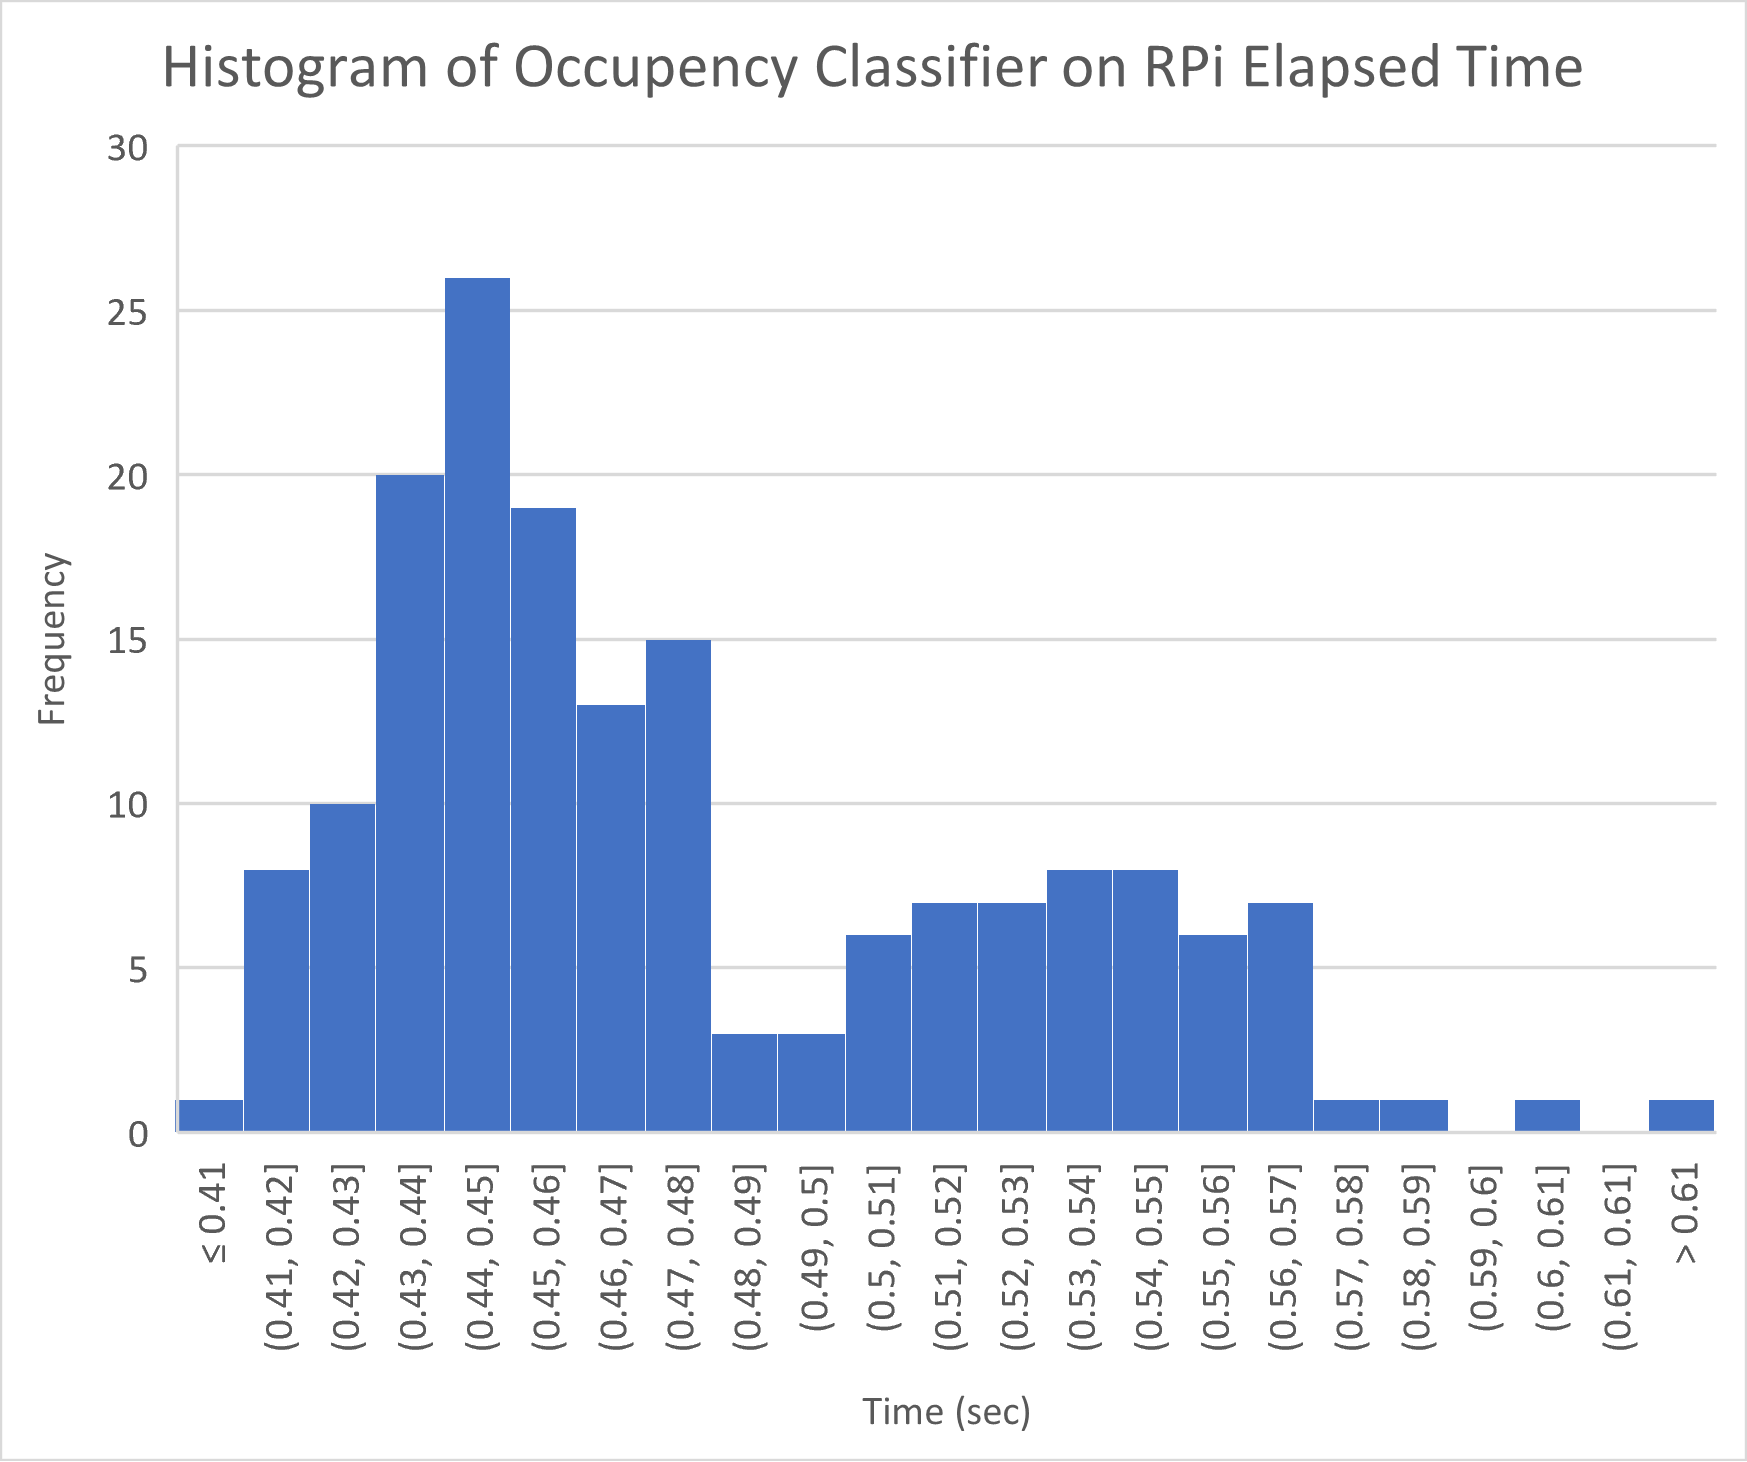
\includegraphics[width=1\textwidth]{VnVReport/OccupencyClassifierPerformance.png}
  \end{center}
\end{figure}


\begin{table}[!h]
\begin{center}
\caption {Occupancy Classifier Summary}
\label{tab:OccClassifierSummary}
\begin{tabular}{ | m{5cm} | m{3cm} | m{3cm} | m{3cm} | } 
\hline
Object Type & Nature & Parking Lot & Occupied (e.g. car, bin, etc.) \\ 
\hline
Total Accuracy & 16/18 & 8/18 & 5/21 \\
\hline
Accuracy on Sunny Conditions & 7/9 & 2/10 & 3/10 \\
\hline
Accuracy on Overcast Conditions & 9/9 & 6/8 & 2/11 \\
\hline
\end{tabular}
\end{center}
\end{table}

\begin{figure}[h!]
  \begin{center} 
  \caption{Sample Images for Sunny Occupied (Left), Sunny Nature (Middle), and Overcast Parking Lot (Right)}
  \label{fig:sampleImages}
        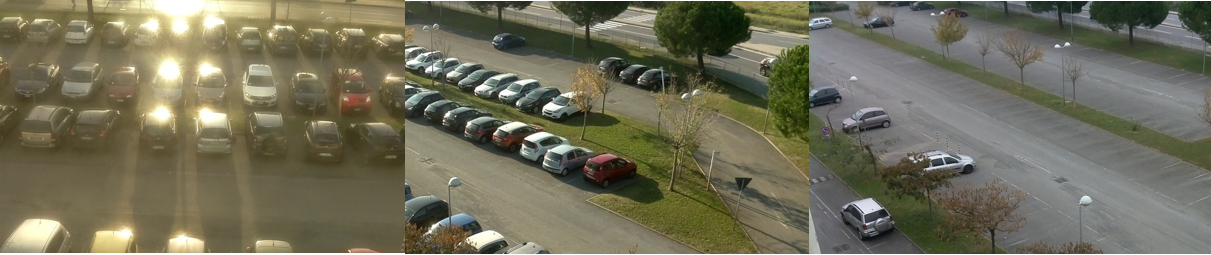
\includegraphics[width=1\textwidth]{VnVReport/SampleImages.png}
  \end{center}
\end{figure}

\begin{table}[!h]
\begin{center}
\caption {UTCR\_012}
\label{tab:UTCR_012}
\begin{tabular}{ | m{3.2cm} | m{12.2cm} | } 
\hline
Test Case Result ID & \nameref{tab:UTCR_012} \\ 
\hline
Test Case Reference & \nameref{tab:UTC_012}  \\ 
\hline
Requirements Tested & \nameref{GEN_001} \\ 
\hline
Procedure & Measure the accuracy of the segmentation algorithm on a satellite imagery dataset of 12. \\ 
\hline
Expected Result & The segmentation algorithm has an average accuracy of above 80\%. Accuracy is calculated as pixels correctly classified divided by the total number of pixels. \\ 
\hline
Actual Result & The segmentation algorithm has an average accuracy of 73\% with a standard deviation of 0.22. Individual results per image are shown in Figure \ref{fig:segAccuracy}. \\ 
\hline
Result Analysis & Fail, the algorithm is well below the 80\% desired. From Figure \ref{fig:segAccuracy}, it can be seen that certain images have much poorer accuracy, such as image 3. The segmented result of image 3 is shown in Figure \ref{fig:segShadow}. The lower half of the image is covered by a shadow from the building, producing a much darker ground surface. This then causes the segmenter to misidentify the parking lot.  \\ 
\hline
\end{tabular}
\end{center}
\end{table}

\begin{figure}[h!]
  \begin{center} 
  \caption{Segmentation Sample: Raw image on left, algorithm segmentation on right (white is parking lot, black is non-parking lot) }
  \label{fig:segResult}
        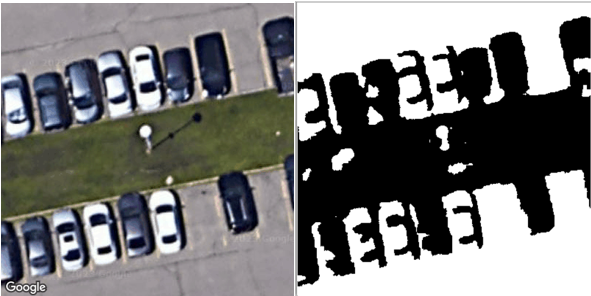
\includegraphics[width=1\textwidth]{VnVReport/SegmentationResult.png}
  \end{center}
\end{figure}

\begin{figure}[h!]
  \begin{center} 
  \caption{Segmentation Accuracy per Image}
  \label{fig:segAccuracy}
        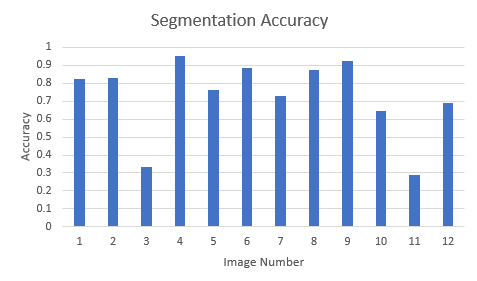
\includegraphics[width=1\textwidth]{VnVReport/SegmentationAccuracy.png}
  \end{center}
\end{figure}

\begin{figure}[h!]
  \begin{center} 
  \caption{Segmentation Result of Image 3 due to Shadow}
  \label{fig:segShadow}
        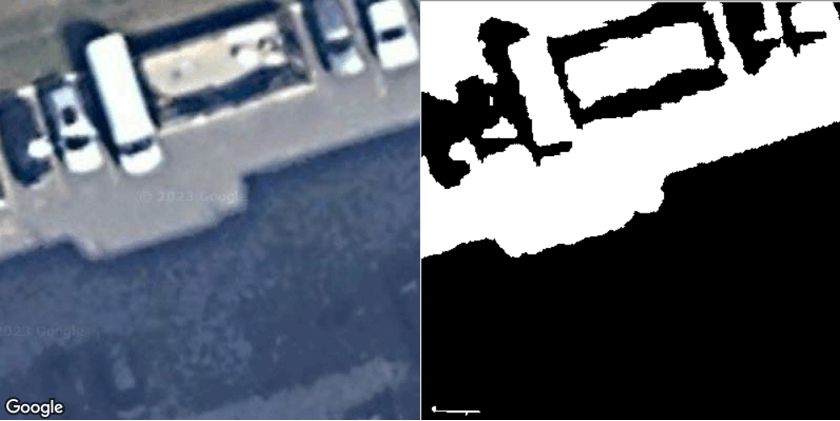
\includegraphics[width=1\textwidth]{VnVReport/SegmentationShadow.png}
  \end{center}
\end{figure}

\clearpage

\subsection{Mapper App}
\label{subsec:mapperApp}

\begin{table}[!h]
\begin{center}
\caption {UTCR\_013}
\label{tab:UTCR_013}
\begin{tabular}{ | m{3.2cm} | m{12.2cm} | } 
\hline
Test Case Result ID & \nameref{tab:UTCR_013} \\ 
\hline
Test Case Reference & \nameref{tab:UTC_013}  \\ 
\hline
Requirements Tested & \nameref{GEN_002}\\ 
\hline
Procedure &  Feed a pre-recorded video of the drone flying over a parking lot into the Vision App. Compare the final occupancy map to the actual occupancy map of the parking lot in the video.\\ 
\hline
Expected Result & The estimated occupancy map should be similar to the actual occupancy in the video. \\ 
\hline
Actual Result & The test was not attempted. \\ 
\hline
Result Analysis & Fail. Occupancy Map creation was a stretch goal for this project, and development for it has not begun. \\ 
\hline
\end{tabular}
\end{center}
\end{table}

\clearpage

\subsection{Path Plan App}
\label{subsec:pathPlanApp}

No unit tests. See \nameref{PathPlanAppUnitTest} for details, and \nameref{sec:SystemTesting} for system tests involving this module.

\subsection{Drone Decision and Control Hiding}
\label{subsec:ddcHiding}

\begin{table}[!h]
\begin{center}
\caption {UTCR\_014}
\label{tab:UTCR_014}
\begin{tabular}{ | m{3.2cm} | m{12.2cm} | } 
\hline
Test Case Result ID & \nameref{tab:UTCR_014} \\ 
\hline
Test Case Reference & \nameref{tab:UTC_014}  \\ 
\hline
Requirements Tested & \nameref{STA_004}, \nameref{GEN_003}, \nameref{TRANS_003}, \nameref{TRANS_015} \\ 
\hline
Procedure & While in the Idle state, send a user command to configure the height parameters to Min\_Hover\_Params. \\ 
\hline
Expected Result & The height params within "Params.txt" and the drone is equal to Min\_Hover\_Params. \\
\hline
Actual Result & The height params within 'Params.txt' and the drone is equal to Min\_Hover\_Params. \\
\hline
Result Analysis & Pass. \\ 
\hline
\end{tabular}
\end{center}
\end{table}

\begin{table}[!h]
\begin{center}
\caption {UTCR\_015}
\label{tab:UTCR_015}
\begin{tabular}{ | m{3.2cm} | m{12.2cm} | } 
\hline
Test Case Result ID & \nameref{tab:UTCR_015} \\ 
\hline
Test Case Reference & \nameref{tab:UTC_015}  \\ 
\hline
Requirements Tested & \nameref{STA_000}, \nameref{STA_001}, \nameref{STA_004}, \nameref{STA_011}, \nameref{STA_012}, \nameref{STA_013}, \nameref{TRANS_003}, \nameref{TRANS_009}, \nameref{TRANS_012}, \nameref{TRANS_013}, \nameref{TRANS_014} \\ 
\hline
Procedure & While in the Idle state, send a user command to arm the drone, takeoff, move 5m to the left, and finally land at the original launch location. \\ 
\hline
Expected Result & The drone arms, takeoffs to the maximum hover height, moves 5m left, and then lands at the original location. \\
\hline
Actual Result & This test is only conducted within the SITL environment. The drone arms, takeoffs to the maximum hover height, moves 5m left, and then lands at the original location. \\
\hline
Result Analysis & Partially pass. The purpose of the test is to verify the drone's ability to takeoff, move, and land autonomously. From the SITL results, it ensures that the behaviour and transitions between the states are meeting specifications. However, real performance on the drone is untested and could suffer performance loses in comparison to SITL. \\ 
\hline
\end{tabular}
\end{center}
\end{table}

\begin{table}[!h]
\begin{center}
\caption {UTCR\_016}
\label{tab:UTCR_016}
\begin{tabular}{ | m{3.2cm} | m{12.2cm} | } 
\hline
Test Case Result ID & \nameref{tab:UTCR_016} \\ 
\hline
Test Case Reference & \nameref{tab:UTC_016}  \\ 
\hline
Requirements Tested & \nameref{STA_009}, \nameref{SR_007}, \nameref{SR_011} \\ 
\hline
Procedure & While in the Idle state, send a user command to arm and takeoff. After a sufficient amount of time, the battery level will drop to 20\% and enter the Malfunction state and lands. \\ 
\hline
Expected Result & The drone takeoffs and hovers until battery capacity reaches 20\%, at which point it enters the Malfunction state and lands. \\
\hline
Actual Result & This test is only conducted within the SITL environment. The drone takeoffs and hovers until battery capacity reaches 20\%, at which point it enters the Malfunction state and lands. \\
\hline
Result Analysis & Principally pass. This test ensures that the Malfunction state and its associated behaviours are correct, and is tested within SITL. \\ 
\hline
\end{tabular}
\end{center}
\end{table}

\begin{table}[!h]
\begin{center}
\caption {UTCR\_017}
\label{tab:UTCR_017}
\begin{tabular}{ | m{3.2cm} | m{12.2cm} | } 
\hline
Test Case Result ID & \nameref{tab:UTCR_017} \\ 
\hline
Test Case Reference & \nameref{tab:UTC_017}  \\ 
\hline
Requirements Tested & \nameref{STA_010}, \nameref{TRANS_010} \\ 
\hline
Procedure & While in the Idle state, send a user command to arm and takeoff. Once max hover height is reached, disconnect the Message Socket. \\ 
\hline
Expected Result & The drone takeoffs and hovers until the Message Socket is disconnected, at which point it enters the Communication Lost state and lands. \\
\hline
Actual Result & Within SITL, drone takeoffs and hovers until the Message Socket is disconnected, at which point it enters the Communication Lost state and lands. When tested on the physical drone, the propellors are removed to prevent flight. The drone enters the Takeoff state and transitions into the Hover state. Once the Message Socket is disconnected, it transitions into the Communication Lost state and attempts to land by decreasing the speed of the motors. \\
\hline
Result Analysis & Principally pass. This test is fully tested within SITL. Within the physical drone, the components related to flight are untested, but the behaviour of the states are verified. \\ 
\hline
\end{tabular}
\end{center}
\end{table}

\begin{table}[!h]
\begin{center}
\caption {UTCR\_018}
\label{tab:UTCR_018}
\begin{tabular}{ | m{3.2cm} | m{12.2cm} | } 
\hline
Test Case Result ID & \nameref{tab:UTCR_018} \\ 
\hline
Test Case Reference & \nameref{tab:UTC_018}  \\ 
\hline
Requirements Tested & \nameref{STA_008}, \nameref{TRANS_008} \\ 
\hline
Procedure & While in the Idle state, send a user command to arm and takeoff. Then send a user command to enter the Autonomous Explore state while no parking lot is detected. \\ 
\hline
Expected Result & After the drone takeoffs, it enters the No Parking Lot Detected Error state. \\
\hline
Actual Result & Within SITL, after the drone takeoffs, it enters the No Parking Lot Detected Error state. When tested on the physical drone, the propellors are removed to prevent flight. The drone enters the takeoff state, and is physically held over a grassy area such that the camera does not see a parking lot. The drone then enters the No Parking Lot Detected Error state. \\
\hline
Result Analysis & Principally pass. This test is fully tested within SITL. Within the physical drone, the components related to flight are untested, but the behaviour of the states are verified. \\ 
\hline
\end{tabular}
\end{center}
\end{table}

\begin{table}[!h]
\begin{center}
\caption {UTCR\_019}
\label{tab:UTCR_019}
\begin{tabular}{ | m{3.2cm} | m{12.2cm} | } 
\hline
Test Case Result ID & \nameref{tab:UTCR_019} \\ 
\hline
Test Case Reference & \nameref{tab:UTC_019}  \\ 
\hline
Requirements Tested & \nameref{STA_003}, \nameref{TRANS_004} \\ 
\hline
Procedure & While in the Idle state, send a user command to arm and takeoff within a parking lot. Hardcode a suggested path of left 5m from the Path Plan App. \\ 
\hline
Expected Result & After the drone takeoffs, it enters the Autonomous Explore state and begins to move left 5m. \\
\hline
Actual Result & Within SITL, after the drone takeoffs within a parking lot, it enters the Autonomous Explore state and begins to move left 5m. This behaviour is not currently tested on the physical drone. \\
\hline
Result Analysis & Principally pass. This test is fully tested within SITL, ensuring correct performance of the Autonomous Explore state. However, it has not yet been tested on the physical drone. \\ 
\hline
\end{tabular}
\end{center}
\end{table}

\clearpage

\subsection{DDC Topic Interface}
\label{subsec:ddcTopicInterface}

\begin{table}[!h]
\begin{center}
\caption {UTCR\_020}
\label{tab:UTCR_020}
\begin{tabular}{ | m{3.2cm} | m{12.2cm} | } 
\hline
Test Case Result ID & \nameref{tab:UTCR_020} \\ 
\hline
Test Case Reference & \nameref{tab:UTC_020}  \\ 
\hline
Requirements Tested & -- \\ 
\hline
Procedure & Provide power to the drone. Hardcode the State Publisher to publish "Unit test 101". Rotate the drone counterclockwise. \\ 
\hline
Expected Result & "Unit test 101" is published on the currStatePub topic. The DDC Topic Interface's readings of the compass values should match that of the readings from a smartphone when rotated. \\
\hline
Actual Result & "Unit test 101" is published on the currStatePub topic. The DDC Topic Interface's readings of the compass values should match that of the readings from a smartphone when rotated. \\
\hline
Result Analysis & Pass. \\ 
\hline
\end{tabular}
\end{center}
\end{table}

\clearpage

\subsection{Algorithm Topic Interface}
\label{subsec:algoTopicInterface}

\begin{table}[!h]
\begin{center}
\caption {UTCR\_021}
\label{tab:UTCR_021}
\begin{tabular}{ | m{3.2cm} | m{12.2cm} | } 
\hline
Test Case Result ID & \nameref{tab:UTCR_021} \\ 
\hline
Test Case Reference & \nameref{tab:UTC_021}  \\ 
\hline
Requirements Tested & -- \\ 
\hline
Procedure & Provide power to the drone. Use the vision app health publisher (visionAppHealth) to publish True. Publish "Unit test 101" on the "current state" topic, and print the drone state being read by the Topic Interface to the console. \\ 
\hline
Expected Result & "Unit test 101" is printed to the console. The visionAppHealth topic is publishing True. \\
\hline
Actual Result & "Unit test 101" is printed to the console. The visionAppHealth topic is publishing True. \\
\hline
Result Analysis & Pass. \\ 
\hline
\end{tabular}
\end{center}
\end{table}

\clearpage

\subsection{DDC Service Interface}
\label{ddcServiceInterface}

\begin{table}[!h]
\begin{center}
\caption {UTCR\_022}
\label{tab:UTCR_022}
\begin{tabular}{ | m{3.2cm} | m{12.2cm} | } 
\hline
Test Case Result ID & \nameref{tab:UTCR_022} \\ 
\hline
Test Case Reference & \nameref{tab:UTC_022}  \\ 
\hline
Requirements Tested & -- \\ 
\hline
Procedure & While in the Idle state, call each of the service routines to set the RtlAlt to 10m, call the mode service to set the mode to "Guided", call the arm service to arm the drone, call the takeoff service to takeoff the drone, and then call the landing service (using the callService_TypeCommand routine). \\ 
\hline
Expected Result & The drone takeoffs from the ground to a height of 10m, and then lands. \\
\hline
Actual Result & Within the SITL environment, the drone takeoffs from the ground to a height of 10m, and then lands. Using the physical drone, the test is changed to set RtlAlt to 1m. The drone then takeoffs to 1m and then lands. However, the landing is rough and the drone flips over during landing. \\
\hline
Result Analysis & Principally pass. The test within SITL verifies that the module is working according to its specifications. However, the physical drone performance regarding landing is lacking, and may be due to the poorly tuned control parameters of the drone. \\ 
\hline
\end{tabular}
\end{center}
\end{table}

\clearpage

\section{Reflection}
\subsection{Project Assessment}
The current quality of the project is inadequate, as the MVP still has yet to be developed. In particular the autonomous flight software not being tuned to fly autonomously is preventing the project from reaching the MVP milestone. However, there has been significant development on meeting some stretch goals, especially those concerned with visual perception. These are shown within \nameref{subsec:visionApp}. 

The most important area of improvement is tuning the flight controller so the drone can attain autonomous flight. Areas such as mechanical, electrical, software infrastructure, and communication network design are developed thoroughly and are fully tested. Therefore, once the flight controller is sufficiently tuned, many of the remaining features will be implemented. Another area of improvement are the visual perception features, in particular improving functionality in sunny weather conditions. The low performance is demonstrated within \nameref{tab:OccClassifierSummary}.

\subsection{Changes Due to Testing}
\label{subsec:changesFromTesting}

The documentation review yielded several important changes that need to be made. Improvements to the SRS included specifying which module implements the height requirement, and requirements need to be written for the design decision to use predownloaded satellite imagery. This includes specifying where satellite imagery is stored on the Operator's PC, specifying how the user can specify a location to download satellite imagery, and what happens when the drone flies in an area without predownloaded satalite imagery. Furthermore, due to changes in design, the definition of c\_CurrentView needs to be changed to be just the live camera view without annotations as opposed to an annotated camera stream. Changes to the FSM are also required as the state machine did not account for when software algorithm modules fail to execute, in addition to the changes made to the compulsive/autonomous move state. The VnV Plan survey also revealed that multiple spare batteries, or larger capacity batteries, should be purchased to facilitate the testing process.

The test cases also revealed issues with the current implementation. For example a visual trace of the drone's previous path in the past 10 seconds is not visible in the GUI, and the accuracy of the visual perception algorithm (both segmentation and classification) is poor and not robust, thus should be improved.

\section{Automated Testing}

Many automated testing tools were used to automate the testing and verification process, as outlined within the \nameref{automatedVerificationTools}. For consistency within the team, VS Code is used as the Integrated Development Environment, with Pylint and clang-tidy for Python and C++ linters respectively. As outlined within \nameref{systemTest} and \nameref{unitTest}, many of the test cases are automatic and are conducted through the UnitTest framework. A list of these automatic test cases are included in Table \ref{tab:automatedTestCases}. In addition to unit testing frameworks, a custom evaluation tool is used to automatically execute and generate metrics for the Vision App test cases, such as within \nameref{tab:OccClassifierSummary}. 

\begin{table}[!h]
\begin{center}
\caption {Automated Test Cases}
\label{tab:automatedTestCases}
\begin{tabular}{ | m{9.2cm} | m{6.2cm} | } 
\hline
Visual Perception and Path Planning & \nameref{tab:STC_015}, \nameref{tab:STC_016} \\ 
\hline
Message Socket & \nameref{tab:UTC_007} \\ 
\hline
Interface Hiding & \nameref{tab:UTC_008}, \nameref{tab:UTC_009}, \nameref{tab:UTC_010} \\ 
\hline
Vision App & \nameref{tab:UTC_011}, \nameref{tab:UTC_012} \\ 
\hline
Mapper App & \nameref{tab:UTC_013} \\ 
\hline
Drone Decision and Control Hiding & \nameref{tab:UTC_014}, \nameref{tab:UTC_015}, \nameref{tab:UTC_016}, \nameref{tab:UTC_017}, \nameref{tab:UTC_018}, \nameref{tab:UTC_019} \\ 
\hline
DDC Topic Interface & \nameref{tab:UTC_020} \\ 
\hline
Algorithm Topic Interface & \nameref{tab:UTC_021} \\ 
\hline
DDC Service Interface & \nameref{tab:UTC_022} \\ 
\hline
\end{tabular}
\end{center}
\end{table}

\clearpage


		
\section{Trace to Requirements}

\begin{table}[!h]
\begin{center}
\caption {FR Traceability Table}
\label{tab:traceTCR_FR}
\begin{tabular}{ | m{3cm} | m{12cm} | } 
\hline
Functional Requirement & Test Case to Verify \\
\hline
\nameref{GEN_001} & \nameref{tab:STCR_014}, \nameref{tab:STCR_016}, \nameref{tab:UTCR_012} \\ \hline
\nameref{GEN_002} & \nameref{tab:STCR_013}, \nameref{tab:STCR_016}, \nameref{tab:UTCR_005}, \nameref{tab:UTCR_006}, \nameref{tab:UTCR_013}\\ \hline
\nameref{GEN_003} & \nameref{tab:STCR_001}, \nameref{tab:STCR_003}, \nameref{tab:UTCR_014} \\ \hline
\nameref{GEN_004} & \nameref{tab:STCR_001}, \nameref{tab:STCR_002} \\ \hline
\nameref{GEN_005} & \nameref{tab:STCR_013}, \nameref{tab:STCR_016}, \nameref{tab:STCR_015}, \nameref{tab:UTCR_011} \\ \hline
\nameref{GEN_006} & \nameref{tab:STCR_013}, \nameref{tab:STCR_016}\\ \hline
\nameref{STA_000} & \nameref{tab:STCR_001}, \nameref{tab:STCR_002}, \nameref{tab:STCR_003}, \nameref{tab:UTCR_015} \\ \hline
\nameref{STA_001} & \nameref{tab:STCR_001}, \nameref{tab:STCR_002}, \nameref{tab:STCR_003}, \nameref{tab:UTCR_015} \\ \hline
\nameref{STA_002} & \nameref{tab:STCR_005}, \nameref{tab:STCR_011} \\ \hline
\nameref{STA_003} & \nameref{tab:STCR_016}, \nameref{tab:STCR_012}, \nameref{tab:STCR_013}, \nameref{tab:UTCR_019} \\ \hline
\nameref{STA_004} & \nameref{tab:STCR_001}, \nameref{tab:STCR_002}, \nameref{tab:STCR_003}, \nameref{tab:UTCR_014}, \nameref{tab:UTCR_015} \\ \hline
\nameref{STA_005} & \nameref{tab:STCR_001}, \nameref{tab:STCR_002}, \nameref{tab:STCR_003} \\ \hline
\nameref{STA_006} & \nameref{tab:STCR_001}, \nameref{tab:STCR_002}, \nameref{tab:STCR_003} \\ \hline
\nameref{STA_007} & \nameref{tab:STCR_011} \\ \hline
\nameref{STA_008} & \nameref{tab:STCR_012}, \nameref{tab:UTCR_018} \\ \hline
\nameref{STA_009} & \nameref{tab:STCR_006}, \nameref{tab:UTCR_016} \\ \hline
\nameref{STA_010} & \nameref{tab:STCR_008}, \nameref{tab:STCR_009}, \nameref{tab:STCR_010}, \nameref{tab:UTCR_017} \\ \hline
\nameref{STA_011} & \nameref{tab:STCR_012}, \nameref{tab:UTCR_015} \\ \hline
\nameref{STA_012} & \nameref{tab:STCR_001}, \nameref{tab:STCR_003} \nameref{tab:UTCR_015} \\ \hline
\nameref{STA_013} & \nameref{tab:STCR_001}, \nameref{tab:STCR_003}, \nameref{tab:UTCR_015} \\ \hline
\end{tabular}
\end{center}
\end{table}

\begin{table}[!h]
\begin{center}
\begin{tabular}{ | m{3cm} | m{12cm} | } 
\hline
Functional Requirement & Test Case to Verify \\
\hline
\nameref{TRANS_001} &  \nameref{tab:STCR_002}, \nameref{tab:STCR_003} \\ \hline
\nameref{TRANS_002} &  \nameref{tab:STCR_001}, \nameref{tab:STCR_002}, \nameref{tab:STCR_003} \\ \hline
\nameref{TRANS_003} & \nameref{tab:STCR_001}, \nameref{tab:STCR_002}, \nameref{tab:STCR_003}, \nameref{tab:UTCR_014}, \nameref{tab:UTCR_015} \\ \hline
\nameref{TRANS_004} & \nameref{tab:STCR_013}, \nameref{tab:STCR_012}, \nameref{tab:UTCR_019} \\ \hline
\nameref{TRANS_005} & \nameref{tab:STCR_004}, \nameref{tab:STCR_011} \\ \hline
\nameref{TRANS_006} & \nameref{tab:STCR_011} \\ \hline
\nameref{TRANS_007} &  \nameref{tab:STCR_012}, \nameref{tab:STCR_013} \\ \hline
\nameref{TRANS_008} & \nameref{tab:STCR_011}, \nameref{tab:UTCR_018} \\ \hline
\nameref{TRANS_009} & \nameref{tab:STCR_001}, \nameref{tab:STCR_002}, \nameref{tab:STCR_003}, \nameref{tab:UTCR_015} \\ \hline
\nameref{TRANS_010} & \nameref{tab:STCR_008}, \nameref{tab:STCR_009}, \nameref{tab:STCR_010}, \nameref{tab:UTCR_017} \\ \hline
\nameref{TRANS_011} & \nameref{tab:STCR_008}, \nameref{tab:STCR_009}, \nameref{tab:STCR_010} \\ \hline
\nameref{TRANS_012} & \nameref{tab:STCR_012}, \nameref{tab:STCR_010}, \nameref{tab:UTCR_015} \\ \hline
\nameref{TRANS_013} & \nameref{tab:STCR_001}, \nameref{tab:STCR_003}, \nameref{tab:UTCR_015} \\ \hline
\nameref{TRANS_014} & \nameref{tab:STCR_001}, \nameref{tab:STCR_003}, \nameref{tab:UTCR_015} \\ \hline
\nameref{TRANS_015} & \nameref{tab:STCR_003}, \nameref{tab:UTCR_014} \\ \hline
\end{tabular}
\end{center}
\end{table}

\begin{table}[!h]
\begin{center}
\caption {NFR Traceability Table}
\label{tab:traceTCR_NFR}
\begin{tabular}{ | m{3cm} | m{12cm} | } 
\hline
Non-Functional Requirement & Test Case to Verify \\
\hline
\nameref{PERF_001} & \nameref{tab:STCR_013} \\ \hline
\nameref{PERF_002} & \nameref{tab:STCR_001}, \nameref{tab:STCR_002}, \nameref{tab:STCR_003} \\ \hline
\nameref{PERF_003} & \nameref{tab:STCR_004} \\ \hline
\nameref{PERF_004} &  \nameref{tab:STCR_013}, \nameref{tab:UTCR_007} \\ \hline
\nameref{PERF_005} & \nameref{tab:STCR_002}, \nameref{tab:STCR_003}, \nameref{tab:UTCR_005}, \nameref{tab:UTCR_006} \\ \hline
\nameref{PERF_006} & \nameref{tab:STCR_004} \\ \hline
\nameref{PERF_007} & \nameref{tab:STCR_015} \\ \hline
\nameref{PERF_008} & \nameref{tab:STCR_004} \\ \hline
\nameref{DES_001} & None, it is a pass or fail depending on components already bought. \\ \hline
\nameref{STD_001} & \nameref{tab:STCR_019} \\ \hline
\nameref{STD_002} & None, it is a pass or fail depending on components already bought. \\ \hline
\nameref{SEC_001} & \nameref{tab:UTCR_009} \\ \hline
\nameref{SEC_002} & None, pass or fail. \\ \hline
\nameref{MTNC_001} & \nameref{tab:STCR_020} \\ \hline
\nameref{MTNC_002} & None, may damage expensive parts. In the interest of cost, this is not tested. \\ \hline
\nameref{MTNC_003} & None, may damage expensive parts. In the interest of cost, this is not tested. \\ \hline
\nameref{SAFE_001} & \nameref{tab:STCR_021} \\ \hline
\nameref{SAFE_002} & \nameref{tab:STCR_002} \\ \hline
\nameref{SAFE_003} & \nameref{tab:STCR_018} \\ \hline
\nameref{SAFE_004} & \nameref{tab:STCR_021} \\ \hline
\nameref{SAFE_005} & None, pass or fail dependent on components bought. \\ \hline
\nameref{USE_001} & \nameref{tab:STCR_004} \\ \hline
\nameref{USE_002} & \nameref{tab:STCR_022} \\ \hline
\nameref{USE_003} & \nameref{tab:STCR_006} \\ \hline
\nameref{USE_004} & \nameref{tab:STCR_017} \\ \hline
\nameref{USE_005} & \nameref{tab:UTCR_008} \\ \hline
\end{tabular}
\end{center}
\end{table}


\begin{table}[!h]
\begin{center}
\begin{tabular}{ | m{3cm} | m{12cm} | } 
\hline
Non-Functional Requirement & Test Case to Verify \\
\hline
\nameref{SR_002} & \nameref{tab:STCR_018}, \nameref{tab:UTCR_008} \\ \hline
\nameref{SR_003} & \nameref{tab:STCR_005}, \nameref{tab:STCR_006} \\ \hline
\nameref{SR_004} & None, pass or fail determined by the components bought. \\ \hline
\nameref{SR_005} & None, pass or fail determined by the components bought. \\ \hline
\nameref{SR_006} & \nameref{tab:STCR_018} \\ \hline
\nameref{SR_007} & \nameref{tab:STCR_010}, \nameref{tab:UTCR_016} \\ \hline
\nameref{SR_008} & None, redundant localization without gps \\ \hline
\nameref{SR_009} & \nameref{tab:STCR_015}, \nameref{tab:STCR_014} \\ \hline
\nameref{SR_010} & \nameref{tab:STCR_018} \\ \hline
\nameref{SR_011} & \nameref{tab:STCR_006}, \nameref{tab:UTCR_016} \\ \hline
\nameref{SR_012} & \nameref{tab:STCR_007} \\ \hline
\nameref{SR_013} & \nameref{tab:UTCR_009} \\ \hline
\end{tabular}
\end{center}
\end{table}


\clearpage
		
\section{Trace to Modules}
This section summarizes the traceability between Test Cases and Modules, see Table \ref{tab:traceTCR_Module}. 


\begin{table}[!h]
\begin{center}
\caption {Traceability Between Test Cases and Modules}
\label{tab:traceTCR_Module}
\begin{tabular}{ | m{5cm} | m{10cm} | }
\hline
Hardware Hiding & \nameref{tab:STCR_001}, \nameref{tab:STCR_002}, \nameref{tab:STCR_003}, \nameref{tab:STCR_004}, \nameref{tab:STCR_005}, \nameref{tab:STCR_006}, \nameref{tab:STCR_007}, \nameref{tab:UTCR_001}, \nameref{tab:UTCR_002}, \nameref{tab:UTCR_003}, \nameref{tab:UTCR_004} \\
\hline
Operator Camera & \nameref{tab:UTCR_005}\\
\hline
Drone Camera &  \nameref{tab:UTCR_006}\\
\hline
Message Socket &  \nameref{tab:STCR_001}, \nameref{tab:STCR_002}, \nameref{tab:STCR_003}, \nameref{tab:STCR_004}, \nameref{tab:STCR_008}, \nameref{tab:STCR_009}, \nameref{tab:STCR_010}, \nameref{tab:UTCR_007}\\
\hline
Interface Hiding &  \nameref{tab:STCR_022}, \nameref{tab:UTCR_008}, \nameref{tab:UTCR_009}, \nameref{tab:UTCR_010}\\
\hline
Vision App &  \nameref{tab:UTCR_011}, \nameref{tab:UTCR_012}\\
\hline
Mapper App &  \nameref{tab:UTCR_013}\\
\hline
Path Plan App & \nameref{tab:UTCR_016} \\
\hline
Drone Decision and Control Hiding &  \nameref{tab:STCR_001}, \nameref{tab:STCR_002}, \nameref{tab:STCR_003}, \nameref{tab:STCR_004}, \nameref{tab:UTCR_014}, \nameref{tab:UTCR_015}, \nameref{tab:UTCR_016}, \nameref{tab:UTCR_017}, \nameref{tab:UTCR_018}, \nameref{tab:UTCR_019} \\
\hline
DDC Topic Interface &  \nameref{tab:STCR_011}, \nameref{tab:STCR_012}, \nameref{tab:UTCR_020}\\
\hline
Algorithm Topic Interface & \nameref{tab:STCR_001}, \nameref{tab:STCR_002}, \nameref{tab:STCR_003}, \nameref{tab:STCR_004}, \nameref{tab:STCR_013}, \nameref{tab:STCR_014}, \nameref{tab:STCR_015}, \nameref{tab:STCR_016}, \nameref{tab:UTCR_021}\\
\hline
DDC Service Interface &  \nameref{tab:UTCR_022}\\
\hline

\end{tabular}
\end{center}
\end{table}		

\section{Symbolic Constants}
See \nameref{tab:symbolic_constants}.

\bibliographystyle{plainnat}
\bibliography{../../refs/References}

\newpage{}
\section*{Appendix --- Reflection}

Verification and Validation (VnV) is a critical process in software development which involves assessing the quality and correctness of the software. The VnV plan outlines the strategies and methodologies that will be employed to verify and validate the software. However, in practice, there may be differences between the VnV plan and the actual VnV activities conducted. These differences may result from unforeseen circumstances, changes in requirements, or other factors.

Many of the test cases involving flight were done within the SITL environment as opposed to with the physical drone. This is due to the incomplete tuning process of the drone, thus preventing autonomous flight. The main cause for the incomplete tuning is due to the extensive damage incurred during testing, and the additional time required to repair and rebuild the drone. However, parallel development continued on the software allowing for nearly all test cases to be tested at least within the SITL environment. Although the extent of damage incurred could not be predicted, additional time could be allocated within the project scheduling for testing to allow a larger buffer for unexpected circumstances.

Another source of change in the VnV Plan is due to the changing requirements, as mentioned within \nameref{subsec:changesFromTesting}. An example would be the change in definition of c\_CurrentView from being an annotated camera stream to an unoannotated one, which was a result of a design change made to simplify the communication infrastructure. Although such changes to the requirements could not be predicted precisely, certain requirements are labeled as requirements likely to change. Thus, test cases involving these requirements could be made with flexibility in mind such that changing the requirement would only require a small change within the test case procedure or expected result.

In conclusion, deviations from the VnV plan are common in software development projects. These deviations may result from changes in requirements, unexpected issues, or other factors. To anticipate changes and minimize the impact of these deviations, project managers must engage in continuous monitoring and evaluation of the development process, regularly review the VnV plan, and remain open to feedback from team members, stakeholders, and end-users.

\end{document}